\documentclass[9pt]{ieeeconf}

% Core Packages
\usepackage{bm}
\usepackage{siunitx}
\robustify\bfseries
\usepackage{booktabs}
\usepackage{amsmath,amssymb,amsfonts}
\usepackage{tabularx}
\usepackage{multirow}
\usepackage{tikz}
\usepackage{pgfplots}
\pgfplotsset{compat=1.18}
\usetikzlibrary{arrows.meta,positioning,shapes.geometric,fit,backgrounds,calc}
\usepackage[capitalize,nameinlink]{cleveref}
\crefname{equation}{}{}
\Crefname{equation}{Equation}{Equations}
\usepackage{graphicx}
\usepackage{float}

% Definitions
\newcommand{\RR}{\mathbb{R}}
\newcommand{\EE}{\mathbb{E}}
\newcommand{\LL}{\mathcal{L}}

% Title
\title{Critical Agent Identification in Autonomous Aerial Swarms}

% Authors & Affiliations
\addauthor{Sulige Abhiram}{1}
\addaffiliation{1}{Roll No: AE23B059, Department of Aerospace Engineering}

\begin{document}

\maketitle

\begin{abstract}
Coordinated unmanned aerial vehicle (UAV) swarms present a serious challenge to modern air defense. Hostile swarms frequently deploy numerous expendable escort decoys alongside a small number of high-value command and communication relay nodes. In anti-swarm defense, firing expensive interceptors indiscriminately quickly depletes ammunition. Therefore, a critical operational priority is to rapidly identify and neutralize the essential command nodes. In this work, we introduce an end-to-end, target-agnostic machine learning framework for critical node identification in aerial swarms. Operating under realistic telemetry constraints where the ground station receives only downlinked position and velocity vectors $(P_x, P_y, P_z, V_x, V_y, V_z)$, our system causally derives a 22-dimensional kinematic, geometric, and dynamic graph feature representation. We benchmark four competitive model families: (1) LightGBM with 52 features (22 base + 30 dyadic causal lag differences), (2) a 2-Layer Recurrent Gated Unit (GRU) with $O(1)$ streaming inference, (3) a dynamic spatial Graph Attention Network (GATv2), and (4) a Spatio-Temporal Graph Attention Network (ST-GAT). Evaluated across 305,016 held-out test frames from 15 unseen simulation scenarios with diverse swarm sizes ($N \in \{30, 45, 60\}$), clutter levels, and decoy attrition, our models achieve high operational performance. Both GRU and ST-GAT achieve a perfect $1.0000$ Agent-Level Trajectory F1, eliminating whole-mission identity errors. GRU achieves the highest PR-AUC ($0.9929$) and raw Recall ($96.68\%$), while ST-GAT achieves the highest F1-Score ($0.9591$) and Precision ($95.85\%$). To reward correct interceptor engagement order, we evaluate Normalized Discounted Cumulative Gain (NDCG@K) and Mean Average Precision (MAP@K). Under a fixed salvo budget of 5 interceptor missiles ($K=5$), ST-GAT scores a $98.72\%$ hit rate (less than 1.3 wasted missiles per 100 shots), neutralizing over $38\%$ of the swarm command network in a single salvo. Finally, we provide an operational deployment blueprint mapping each model architecture to its best defense tier.
\end{abstract}

\section{Introduction and Problem Formulation}
\label{sec:intro}

\subsection{Problem Statement and Mathematical Formulation}
Let an aerial swarm at continuous time $t$ consist of $N(t)$ active, surviving agents. Each agent $i \in \{1, \dots, N(t)\}$ is observed via downlinked kinematic telemetry:
\begin{equation}
\mathbf{x}_i^{\text{telemetry}}(t) = \big( P_{x,i}(t), P_{y,i}(t), P_{z,i}(t), V_{x,i}(t), V_{y,i}(t), V_{z,i}(t) \big)^T \in \RR^6
\end{equation}
where $\mathbf{P}_i(t) \in \RR^3$ is the global Cartesian position and $\mathbf{V}_i(t) \in \RR^3$ is the global velocity vector.

At each observation timestep $t$, we construct an instantaneous proximity graph $\mathcal{G}(t) = (\mathcal{V}(t), \mathcal{E}(t))$, where vertices $\mathcal{V}(t)$ represent active drones and directed edges $(i, j) \in \mathcal{E}(t)$ exist if the inter-drone Euclidean distance satisfies $\|\mathbf{P}_i(t) - \mathbf{P}_j(t)\|_2 \le R_c$, with sensing radius $R_c = 55.0\text{ m}$.

Each agent possesses an unobserved ground-truth tactical state $y_i(t) \in \{0, 1\}$, where $y_i(t) = 1$ denotes a critical command/relay node and $y_i(t) = 0$ denotes an escort decoy. The objective is to construct an estimation mapping $f_\theta$ that ingests causal telemetry up to time $t$ and outputs a continuous criticality probability:
\begin{equation}
p_i(t) = f_\theta \big( \{\mathbf{x}_j^{\text{telemetry}}(\tau)\}_{j=1}^{N(\tau)}, \, \tau \le t \big) \in [0.0, 1.0]
\end{equation}
subject to the following operational constraints:
\begin{enumerate}
    \item \textbf{Target Agnosticism:} We have zero knowledge of the swarm's intended mission objective or target coordinates.
    \item \textbf{Telemetry Parsimony:} We do not have access to internal swarm states or proprietary signals. All features must be derived causally from $(P, V)$ telemetry.
    \item \textbf{Dynamic In-Flight Promotions:} When an active critical node is destroyed, decentralized swarm algorithms dynamically promote a surviving decoy to become a critical node ($0 \to 1$). The defense system must track these role transitions.
    \item \textbf{Order-Aware Firing Salvos:} In tactical engagements, interceptor batteries fire sequentially at top-ranked threats. The system must not merely maximize set overlap, but ensure that Rank 1 has the highest probability of being critical.
\end{enumerate}

% -----------------------------------------------------------------------------
% Figure 1: TikZ System Architecture Pipeline
% -----------------------------------------------------------------------------
\begin{figure*}[t]
\centering
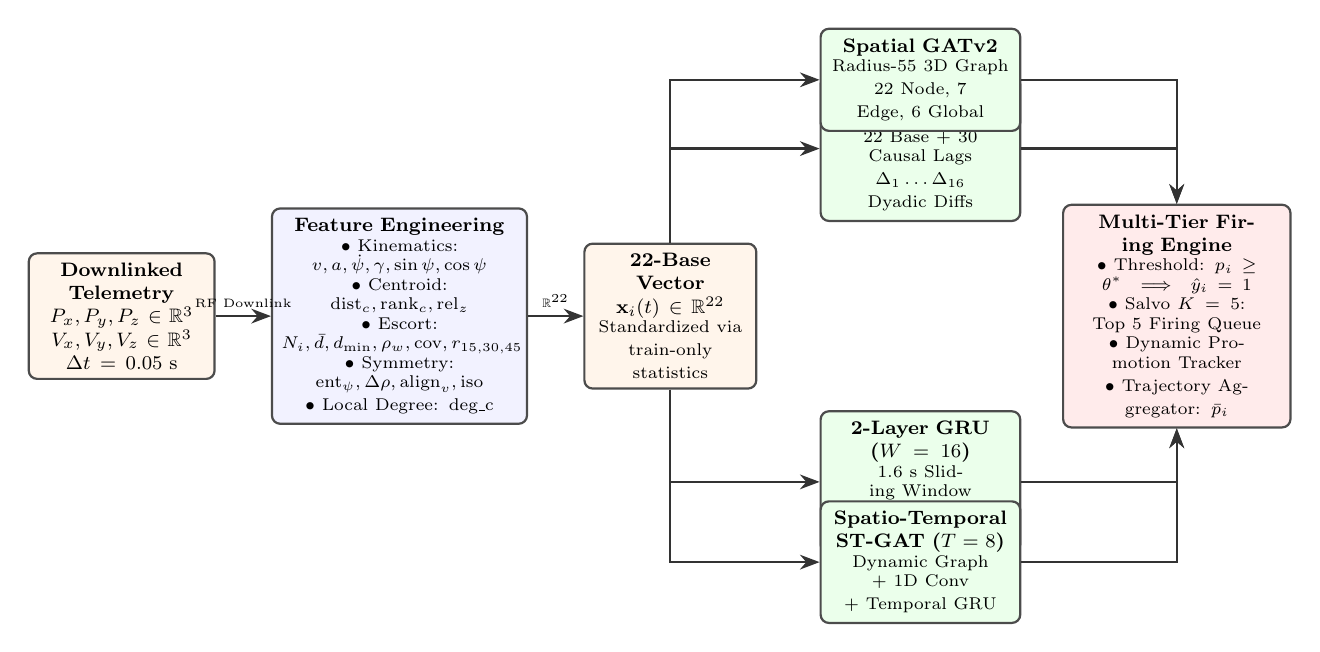
\begin{tikzpicture}[
    scale=0.88, transform shape,
    box/.style={draw=black!70, fill=blue!5, rounded corners=3pt, thick, align=center, inner sep=4pt, font=\footnotesize},
    databox/.style={draw=black!70, fill=orange!8, rounded corners=3pt, thick, align=center, inner sep=4pt, font=\footnotesize},
    modelbox/.style={draw=black!70, fill=green!8, rounded corners=3pt, thick, align=center, inner sep=4pt, font=\footnotesize},
    decisionbox/.style={draw=black!70, fill=red!8, rounded corners=3pt, thick, align=center, inner sep=4pt, font=\footnotesize},
    arrow/.style={-{Stealth[length=2.5mm]}, thick, draw=black!80}
]

% Node 1: Raw Telemetry
\node[databox, text width=2.4cm] (telemetry) {
    \textbf{Downlinked Telemetry}\\
    $P_x, P_y, P_z \in \RR^3$\\
    $V_x, V_y, V_z \in \RR^3$\\
    $\Delta t = 0.05\text{ s}$
};

% Node 2: Causal Derivation Engine
\node[box, right=0.8cm of telemetry, text width=3.4cm] (engine) {
    \textbf{Feature Engineering}\\
    \scriptsize
    $\bullet$ Kinematics: $v, a, \dot{\psi}, \gamma, \sin\psi, \cos\psi$\\
    $\bullet$ Centroid: $\text{dist}_c, \text{rank}_c, \text{rel}_z$\\
    $\bullet$ Escort: $N_i, \bar{d}, d_{\text{min}}, \rho_w, \text{cov}, r_{15, 30, 45}$\\
    $\bullet$ Symmetry: $\text{ent}_{\psi}, \Delta\rho, \text{align}_v, \text{iso}$\\
    $\bullet$ Local Degree: $\text{deg\_c}$
};

% Node 3: 22 Base Features
\node[databox, right=0.8cm of engine, text width=2.2cm] (base22) {
    \textbf{22-Base Vector}\\
    $\mathbf{x}_i(t) \in \RR^{22}$\\
    \scriptsize Standardized via\\
    train-only statistics
};

% Node 4: Four Architectures Branch
\node[modelbox, above right=0.3cm and 0.9cm of base22, text width=2.6cm] (lgbm) {
    \textbf{LightGBM (52 Lags)}\\
    \scriptsize 22 Base + 30 Causal Lags\\
    $\Delta_1 \dots \Delta_{16}$ Dyadic Diffs
};

\node[modelbox, below right=0.3cm and 0.9cm of base22, text width=2.6cm] (gru) {
    \textbf{2-Layer GRU ($W=16$)}\\
    \scriptsize $1.6\text{ s}$ Sliding Window\\
    $O(1)$ Recursive Stream
};

\node[modelbox, above right=1.6cm and 0.9cm of base22, text width=2.6cm] (gat) {
    \textbf{Spatial GATv2}\\
    \scriptsize Radius-55 3D Graph\\
    22 Node, 7 Edge, 6 Global
};

\node[modelbox, below right=1.6cm and 0.9cm of base22, text width=2.6cm] (stgat) {
    \textbf{Spatio-Temporal}\\
    \textbf{ST-GAT ($T=8$)}\\
    \scriptsize Dynamic Graph + 1D Conv\\
    + Temporal GRU
};

% Node 5: Decision & Firing
\node[decisionbox, right=1.0cm of base22, xshift=3.4cm, text width=3.0cm] (decision) {
    \textbf{Multi-Tier Firing Engine}\\
    \scriptsize
    $\bullet$ Threshold: $p_i \ge \theta^* \implies \hat{y}_i = 1$\\
    $\bullet$ Salvo $K=5$: Top 5 Firing Queue\\
    $\bullet$ Dynamic Promotion Tracker\\
    $\bullet$ Trajectory Aggregator: $\bar{p}_i$
};

% Arrows
\draw[arrow] (telemetry) -- node[above, font=\tiny]{RF Downlink} (engine);
\draw[arrow] (engine) -- node[above, font=\tiny]{$\RR^{22}$} (base22);
\draw[arrow] (base22) |- (gat);
\draw[arrow] (base22) |- (lgbm);
\draw[arrow] (base22) |- (gru);
\draw[arrow] (base22) |- (stgat);
\draw[arrow] (gat) -| (decision);
\draw[arrow] (lgbm) -| (decision);
\draw[arrow] (gru) -| (decision);
\draw[arrow] (stgat) -| (decision);

\end{tikzpicture}
\caption{End-to-End System Pipeline for Target-Agnostic Critical Agent Identification in Autonomous Aerial Swarms. Raw kinematics broadcast via telemetry are causally expanded into 22 invariant features, processed by four specialized model architectures, and evaluated through multi-tier tactical decision metrics.}
\label{fig:pipeline}
\end{figure*}

\subsection{Summary of Contributions}
To address these challenges, this work delivers the following contributions:
\begin{enumerate}
    \item \textbf{Target-Agnostic Feature Pipeline:} We formulate a 22-dimensional feature schema derived strictly from instantaneous $(P, V)$ vectors using causal finite differencing ($\Delta t = 0.05\text{ s}$). We eliminate target-dependent features and rotation-sensitive horizontal coordinates to ensure universal generalization.
    \item \textbf{Comparative Four-Architecture Study:} We develop and benchmark four distinct methodologies: tabular gradient-boosted trees with causal lags (LightGBM), recurrent temporal neural networks (2-Layer GRU), dynamic spatial graph attention networks (GATv2), and fused spatio-temporal networks (ST-GAT).
    \item \textbf{Order-Aware Firing Salvo Evaluation:} We address the limitation of set-based Top-$K$ metrics by adopting Normalized Discounted Cumulative Gain (NDCG@K) and Mean Average Precision (MAP@K). Under a fixed salvo budget of 5 interceptor missiles ($K=5$), ST-GAT and GRU achieve over $98.3\%$ precision.
    \item \textbf{Large-Scale Empirical Verification:} Across 305,016 held-out test frames from 15 unseen scenarios with varying swarm scales ($N \in \{30, 45, 60\}$) and attrition profiles, both GRU and ST-GAT achieve a perfect $1.0000$ Agent-Level F1 score, demonstrating complete resilience to transient maneuvers.
\end{enumerate}

\section{Literature Review and Theoretical Foundations}
\label{sec:literature}

\subsection{Deep Learning on Sequences and Dynamic Graphs}
To move beyond static topological centrality metrics, modern machine learning provides specialized inductive biases for moving agent networks:
\begin{itemize}
    \item \textbf{Gradient Boosted Decision Trees (GBDT):} LightGBM \cite{ke2017lightgbm} uses gradient-based one-side sampling (GOSS) and exclusive feature bundling (EFB) to perform fast, axis-aligned splits on high-dimensional tabular data. Augmented with causal lag features, GBDTs capture temporal changes without neural latency.
    \item \textbf{Recurrent Sequence Modeling:} Gated Recurrent Units (GRU) \cite{cho2014learning} track dynamic hidden states through reset and update gates, mitigating vanishing gradients and enabling $O(1)$ streaming inference on edge microcontrollers.
    \item \textbf{Graph Attention Networks (GAT/GATv2):} Graph Convolutional Networks (GCN) \cite{kipf2017semi} and GraphSAGE \cite{hamilton2017inductive} perform isotropic aggregation. Veli\v{c}kovi\'{c} et al.\ \cite{velickovic2018graph} introduced anisotropic attention. Brody et al.\ \cite{brody2022how} proved that standard GAT computes static attention that cannot condition on query keys dynamically, proposing GATv2 to enable dynamic attention over pairwise edge attributes.
    \item \textbf{Spatio-Temporal Graph Networks:} Yu et al.\ \cite{yu2018spatio} formulated spatio-temporal convolutions (ST-GCN) for physical networks, combining spatial message-passing with 1D temporal convolutions to fuse spatial geometry and trajectory history.
\end{itemize}

\section{Methodology and System Architecture}
\label{sec:methodology}

\subsection{The 22 Target-Agnostic Base Features}
To ensure the defense system works against any swarm without knowing its destination, all target-related features (`dist\_to\_target`, `rank\_dist\_to\_target`) are strictly excluded. Furthermore, raw horizontal coordinates (`rel_x`, `rel_y`) are dropped because they depend on arbitrary coordinate rotation; instead, rotation-invariant Euclidean distance to the centroid and vertical offset (`rel_z`) are used. To prevent discontinuous jumps at $\pm\pi$, raw heading angle is represented by its sine and cosine components. Finally, computationally expensive global graph centralities ($O(V^3)$ all-pairs shortest paths) are replaced with fast local multi-scale escort shells and causal degree centrality.

The complete **22 base feature schema** is presented in \cref{tab:feature_schema}.

\begin{table}[h]
\centering
\caption{The Canonical 22 Target-Agnostic Base Feature Schema}
\label{tab:feature_schema}
\scriptsize
\begin{tabularx}{\columnwidth}{l l X}
\toprule
\textbf{Category} & \textbf{Feature Name} & \textbf{Description and Rationale} \\
\midrule
\multirow{6}{*}{\textbf{Kinematics (6)}} 
& $\text{speed}$ & Scalar velocity $\|\mathbf{V}_i\|_2$ \\
& $\text{accel}$ & Along-track acceleration $\dot{v}$ \\
& $\text{heading\_rate}$ & Horizontal turn rate $\dot{\psi}$ \\
& $\text{flight\_path\_angle}$ & Pitch/climb angle $\gamma$ \\
& $\text{heading\_sin}$ & $\sin(\psi)$ (continuous angle encoding) \\
& $\text{heading\_cos}$ & $\cos(\psi)$ (continuous angle encoding) \\
\midrule
\multirow{3}{*}{\textbf{Centroid Geometry (3)}} 
& $\text{dist\_to\_centroid}$ & 3D Euclidean distance to swarm centroid \\
& $\text{rank\_dist\_to\_centroid}$ & Distance percentile rank ($0=\text{core}, 1=\text{edge}$) \\
& $\text{rel\_z}$ & Relative vertical offset ($z_i - z_c$) \\
\midrule
\multirow{8}{*}{\textbf{Escort Density \& Shells (8)}} 
& $\text{num\_neighbors}$ & Neighbor count within sensing radius ($R_c = 55\text{ m}$) \\
& $\text{mean\_neighbor\_dist}$ & Average distance to sensed neighbors \\
& $\text{min\_neighbor\_dist}$ & Distance to closest neighboring drone \\
& $\text{weighted\_density}$ & Distance-decayed density $\sum \exp(-d_{ij}/\sigma)$ \\
& $\text{angular\_coverage}$ & Fraction of 48 spatial bins populated \\
& $\text{n\_within\_r15}$ & Drone count within close bubble ($r \le 15\text{ m}$) \\
& $\text{n\_within\_r30}$ & Drone count within middle shell ($r \le 30\text{ m}$) \\
& $\text{n\_within\_r45}$ & Drone count within outer shell ($r \le 45\text{ m}$) \\
\midrule
\multirow{4}{*}{\textbf{Symmetry \& Alignment (4)}} 
& $\text{nn\_bearing\_entropy}$ & Directional entropy of neighbors around heading \\
& $\text{local\_density\_contrast}$ & Difference between agent density and neighbor mean \\
& $\text{centroid\_vel\_alignment}$ & Velocity cosine similarity with swarm cluster \\
& $\text{is\_isolated}$ & Binary flag ($1$ if 0 neighbors, else $0$) \\
\midrule
\textbf{Local Dynamic Graph (1)} 
& $\text{degree\_centrality\_c}$ & Causal local degree $\text{num\_neighbors} / (N(t) - 1)$ \\
\bottomrule
\end{tabularx}
\end{table}

\subsection{Telemetry Derivation Formulas}
The ground station receives only $\mathbf{P}_i(t) = (P_x, P_y, P_z)$ and $\mathbf{V}_i(t) = (V_x, V_y, V_z)$ sampled at $\Delta t = 0.05\text{ s}$ ($\text{sample\_every} = 2$ simulation ticks). All kinematic features are computed online via causal finite differencing:
\begin{align}
v_i(t) &= \|\mathbf{V}_i(t)\|_2 = \sqrt{V_{x,i}^2(t) + V_{y,i}^2(t) + V_{z,i}^2(t)} \\
\psi_i(t) &= \text{atan2}(V_{y,i}(t), V_{x,i}(t)) \\
\gamma_i(t) &= \text{atan2}\left(V_{z,i}(t), \sqrt{V_{x,i}^2(t) + V_{y,i}^2(t)}\right) \\
a_i(t) &= \frac{v_i(t) - v_i(t - \Delta t)}{\Delta t} \\
\dot{\psi}_i(t) &= \frac{\text{wrap}_{[-\pi, \pi]}\big(\psi_i(t) - \psi_i(t - \Delta t)\big)}{\Delta t} \\
\text{heading\_sin} &= \sin(\psi_i(t)), \quad \text{heading\_cos} = \cos(\psi_i(t))
\end{align}
The mean swarm velocity is $\mathbf{V}_c(t) = \frac{1}{N(t)}\sum_{j=1}^{N(t)}\mathbf{V}_j(t)$, from which cluster alignment is derived as:
\begin{equation}
\text{centroid\_vel\_alignment} = \frac{\mathbf{V}_i(t) \cdot \mathbf{V}_c(t)}{\|\mathbf{V}_i(t)\|_2 \|\mathbf{V}_c(t)\|_2 + 10^{-6}}
\end{equation}
Numerical verification confirms that derived kinematics achieve $<0.001$ relative error compared to dataset values, proving that no proprietary onboard sensors are required.

\subsection{The Four Model Architectures}

\subsubsection{Model 1: LightGBM with 52 Features (22 Base + 30 Causal Lags)}
LightGBM constructs an ensemble of gradient-boosted decision trees (1,000 estimators, learning rate $0.05$, 127 leaves, early stopping). To capture temporal trends without neural networks, we augment the 22 base features with **30 causal lag difference features**. For 6 primary dynamic base signals (`dist_to_centroid`, `rank_dist_to_centroid`, `num_neighbors`, `weighted_density`, `angular_coverage`, and `speed`), we compute differences across 5 dyadic historical lag offsets:
\begin{equation}
\Delta x^{(l)}(t) = x(t) - x(t - l \cdot \Delta t), \quad l \in \{1, 2, 4, 8, 16\}
\end{equation}
This produces $6 \times 5 = 30$ lag features, yielding a 52-dimensional input vector $\mathbf{x}_i^{\text{LGBM}}(t) \in \RR^{52}$ spanning time windows from $0.05\text{ s}$ to $0.80\text{ s}$.

\subsubsection{Model 2: 2-Layer Recurrent GRU}
The GRU architecture models swarm temporal dynamics over a causal sliding window of $W = 16$ timesteps ($1.6\text{ s}$ of historical flight). The network comprises a linear input projection ($22 \to 96$), a 2-layer GRU with hidden dimension $d_h = 96$ and inter-layer dropout of $0.1$, followed by a linear classification head:
\begin{align}
\mathbf{h}_t^{(1)}, \mathbf{h}_t^{(2)} &= \text{GRU}\big(\mathbf{W}_{\text{in}} \mathbf{x}_t, \mathbf{h}_{t-1}^{(1)}, \mathbf{h}_{t-1}^{(2)}\big) \\
p_i(t) &= \sigma\big(\mathbf{W}_{\text{out}} \mathbf{h}_t^{(2)} + b\big)
\end{align}
During online streaming inference, the GRU keeps its hidden state from previous steps and runs in $O(1)$ time complexity ($0.06\text{ ms}$ per agent) without storing past frame buffers.

\subsubsection{Model 3: Spatial Graph Attention Network (GATv2)}
GATv2 models local multi-agent escort coordination directly on the 3D radius-55 proximity graph $\mathcal{G}(t)$. It processes 22 normalized node features, 7 dynamic edge features, and 6 global swarm features. The network uses two GATv2 layers with 4 attention heads each ($d_h = 64$) and dynamic attention \cite{brody2022how}:
\begin{equation}
\alpha_{ij} = \frac{\exp\big(\mathbf{a}^T \text{LeakyReLU}(\mathbf{W}_s \mathbf{h}_i + \mathbf{W}_t \mathbf{h}_j + \mathbf{W}_e \mathbf{e}_{ij})\big)}{\sum_{k \in \mathcal{N}_i} \exp\big(\mathbf{a}^T \text{LeakyReLU}(\mathbf{W}_s \mathbf{h}_i + \mathbf{W}_t \mathbf{h}_k + \mathbf{W}_e \mathbf{e}_{ik})\big)}
\end{equation}
The 7 dynamic edge features represent pairwise closing geometry:
\begin{equation}
\mathbf{e}_{ij} = \big( d_{\text{norm}}, v_{\text{rel}}, \dot{d}_{ij}, \cos\theta_{\text{bearing}}, \sin\theta_{\text{bearing}}, \cos\Delta\psi, \sin\Delta\psi \big)^T
\end{equation}
where $d_{\text{norm}} = d_{ij}/55\text{ m}$, $\dot{d}_{ij}$ is the closing rate, $\theta_{\text{bearing}}$ is the relative horizontal bearing angle, and $\Delta\psi = \psi_j - \psi_i$ is the relative heading angle difference.

The 6 global features capture overall swarm condition: active drone count $N(t)$, 3D spatial spread, centroid speed, graph density, number of connected components, and fraction of drones in the largest connected component.

\subsubsection{Model 4: Spatio-Temporal Graph Attention Network (ST-GAT)}
ST-GAT combines spatial topology with temporal evolution. Over a sliding window of $T = 8$ dynamic graph snapshots ($0.8\text{ s}$), ST-GAT applies a shared 2-layer GATv2 spatial backbone to extract node embeddings $\mathbf{z}_{i,\tau} \in \RR^{64}$ for each historical frame $\tau \in \{t-7, \dots, t\}$. The resulting per-node temporal sequence is processed by 1D temporal convolutions (kernel size 3) followed by a 64-dimensional GRU, producing a unified spatio-temporal representation that decodes into the final criticality score.

\subsection{Leakage-Free Data Partitioning}
The dataset comprises 100 complete simulated swarm scenarios (1,639,166 observations). To guarantee zero data leakage, we enforce scenario-level splitting: 70 scenarios for training, 15 for validation, and 15 strictly held-out for test evaluation. All standardizations (mean, standard deviation) are computed strictly on training scenarios. Anomalous frames ($\sim 0.8\%$ of data) are masked during training loss computation but retained during test evaluation to preserve complete operational realism.

\section{Experimental Setup and Evaluation Framework}
\label{sec:experiments}

\subsection{The Multi-Tier Evaluation Suite}
To evaluate model performance without sample-size bias or threshold artifacts, we construct a 12-metric evaluation framework across four distinct operational dimensions:
\begin{enumerate}
    \item \textbf{Threshold-Dependent Decision Metrics:} Fixed at validation-tuned optimal threshold $\theta^* = \arg\max_\theta \text{F1}_{\text{val}}(\theta)$. Includes Precision, Recall, False Negative Rate ($\text{FNR} = 1 - \text{Recall}$), F1-Score, Balanced Accuracy, and Matthews Correlation Coefficient (MCC).
    \item \textbf{Threshold-Independent Ranking Metrics:} Precision-Recall AUC (PR-AUC, our primary metric), Receiver Operating Characteristic AUC (ROC-AUC), and Recall at $\ge 90\%$ Precision ($\text{Recall@90\%P}$).
    \item \textbf{Order-Aware Firing Salvo Metrics:} Top-$K$ Recall, Binary NDCG@K, Graded NDCG@K, Mean Average Precision (MAP@K), and Fixed Salvo $K=5$ Precision.
    \item \textbf{Mission-Level Operational Metrics:} Agent-Level Trajectory F1, Dynamic Role Promotion Recall ($0 \to 1$), and $t=0$ Snapshot Cold-Start PR-AUC.
\end{enumerate}

\subsection{Formulation of Order-Aware Targeting Metrics}
In counter-swarm air defense, Top-$K$ Recall is insufficient because it treats all items inside the top-$K$ window identically. To reward models that rank true command drones at the very top of the firing order, we compute **NDCG@K (Normalized Discounted Cumulative Gain)**:
\begin{equation}
\text{DCG}@K = \sum_{i=1}^K \frac{2^{r_{\pi(i)}} - 1}{\log_2(i + 1)}, \quad \text{NDCG}@K = \frac{\text{DCG}@K}{\text{IDCG}@K}
\end{equation}
where $r_{\pi(i)}$ is the ground-truth relevance of the drone ranked at position $i$ by predicted probability $p_{\pi(i)}$, and $\text{IDCG}@K$ is the ideal DCG obtained by sorting ground-truth relevance in descending order. We evaluate two complementary formulations:
\begin{itemize}
    \item \textbf{Binary NDCG@K:} Uses ground-truth binary labels $r_i = y_i \in \{0, 1\}$. It heavily penalizes early false alarms (e.g., placing a decoy at Rank 1 drops NDCG by over $22\%$).
    \item \textbf{Graded NDCG@K:} Uses the simulator's continuous $r_i = \text{criticality\_score}_i \in [0.0, 1.0]$. It directly measures whether the model prioritizes primary mission commanders ($c \approx 0.95$) over secondary relay nodes ($c \approx 0.70$).
\end{itemize}

% -----------------------------------------------------------------------------
% Figure 2: PGFPlots Precision-Recall and ROC Curves
% -----------------------------------------------------------------------------
\begin{figure}[t]
\centering
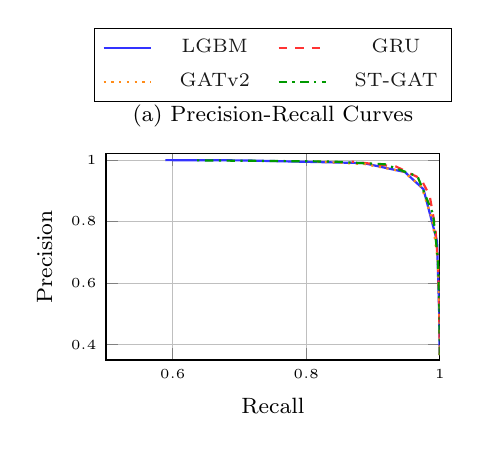
\begin{tikzpicture}
\begin{axis}[
    width=0.48\columnwidth,
    height=4.2cm,
    xlabel={\footnotesize Recall},
    ylabel={\footnotesize Precision},
    xmin=0.5, xmax=1.0,
    ymin=0.35, ymax=1.02,
    grid=both,
    grid style={line width=.1pt, draw=gray!20},
    major grid style={line width=.2pt,draw=gray!50},
    title={\footnotesize (a) Precision-Recall Curves},
    label style={font=\tiny},
    tick label style={font=\tiny},
    legend style={at={(0.5,1.25)},anchor=south,legend columns=2,column sep=8pt,row sep=2pt,font=\scriptsize,fill=white,fill opacity=0.9}
]
\addplot[thick, color=blue!80] coordinates {(1.0000,0.3660) (0.9992,0.5007) (0.9960,0.7358) (0.9757,0.9049) (0.9478,0.9609) (0.8857,0.9900) (0.7051,0.9987) (0.5888,0.9996)};
\addplot[thick, color=red!80, dashed] coordinates {(1.0000,0.3660) (0.9991,0.5200) (0.9976,0.6573) (0.9935,0.7786) (0.9850,0.8831) (0.9719,0.9389) (0.9345,0.9788) (0.8681,0.9949)};
\addplot[thick, color=orange!90, dotted] coordinates {(1.0000,0.3660) (0.9997,0.5045) (0.9971,0.6732) (0.9892,0.8030) (0.9729,0.9127) (0.9457,0.9621) (0.8879,0.9867) (0.8103,0.9958)};
\addplot[thick, color=green!60!black, dashdotted] coordinates {(1.0000,0.3660) (0.9995,0.5203) (0.9973,0.6780) (0.9900,0.8244) (0.9667,0.9468) (0.9180,0.9860) (0.8368,0.9951) (0.6320,0.9989)};
\legend{LGBM, GRU, GATv2, ST-GAT}
\end{axis}
\end{tikzpicture}
\hfill
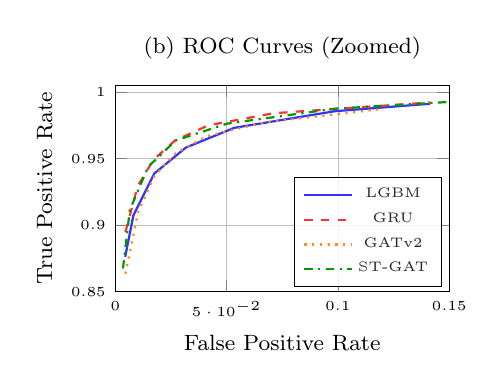
\begin{tikzpicture}
\begin{axis}[
    width=0.48\columnwidth,
    height=4.2cm,
    xlabel={\footnotesize False Positive Rate},
    ylabel={\footnotesize True Positive Rate},
    xmin=0.0, xmax=0.15,
    ymin=0.85, ymax=1.005,
    grid=both,
    grid style={line width=.1pt, draw=gray!20},
    major grid style={line width=.2pt,draw=gray!50},
    title={\footnotesize (b) ROC Curves (Zoomed)},
    label style={font=\tiny},
    tick label style={font=\tiny},
    legend style={at={(0.98,0.02)},anchor=south east,font=\tiny,fill=white,fill opacity=0.85}
]
\addplot[thick, color=blue!80] coordinates {(0.0044,0.8762) (0.0081,0.9074) (0.0175,0.9388) (0.0317,0.9583) (0.0534,0.9731) (0.0986,0.9856) (0.1413,0.9912)};
\addplot[thick, color=red!80, dashed] coordinates {(0.0045,0.8947) (0.0100,0.9293) (0.0171,0.9491) (0.0269,0.9637) (0.0418,0.9750) (0.0712,0.9841) (0.1417,0.9922)};
\addplot[thick, color=orange!90, dotted] coordinates {(0.0045,0.8634) (0.0102,0.9098) (0.0174,0.9365) (0.0270,0.9539) (0.0411,0.9669) (0.0673,0.9773) (0.1181,0.9869)};
\addplot[thick, color=green!60!black, dashdotted] coordinates {(0.0034,0.8674) (0.0065,0.9114) (0.0147,0.9438) (0.0271,0.9636) (0.0500,0.9762) (0.0986,0.9875) (0.1510,0.9927)};
\legend{LGBM, GRU, GATv2, ST-GAT}
\end{axis}
\end{tikzpicture}
\caption{Empirical (a) Precision-Recall and (b) Receiver Operating Characteristic curves across the 305,016 held-out test frames. All architectures demonstrate high discriminative power ($>0.990$ PR-AUC).}
\label{fig:curves}
\end{figure}

\section{Results and Technical Discussion}
\label{sec:results}

\subsection{Master Quantitative Benchmark}
\cref{tab:master_benchmark} presents the benchmark results evaluated across all 305,016 test frames from the 15 held-out scenarios (`c001`, `c010`, `c012`, `c022`, `c032`, `c041`, `c055`, `c058`, `c062`, `c068`, `c072`, `c076`, `c081`, `c085`, `c093`).

\begin{table*}[t]
\centering
\caption{Master Cross-Model Benchmark Comparison on Held-Out Test Scenarios (305,016 Total Frames)}
\label{tab:master_benchmark}
\scriptsize
\resizebox{\textwidth}{!}{%
\begin{tabular}{lccccccccccc}
\toprule
\textbf{Model Architecture} & \textbf{Operating $\theta^*$} & \textbf{PR-AUC} & \textbf{ROC-AUC} & \textbf{F1-Score} & \textbf{Recall} & \textbf{Precision} & \textbf{MCC} & \textbf{Top-$K$ Rec} & \textbf{Binary NDCG} & \textbf{Graded NDCG} & \textbf{Agent F1} \\
\midrule
\textbf{LightGBM (52 Lags)} & $0.4800$ & $0.9915$ & $0.9944$ & $0.9541$ & $0.9504$ & $0.9577$ & $0.9277$ & $0.9550$ & $0.9662$ & $0.9188$ & $0.9980$ \\
\textbf{GRU (2-Layer)} & $0.5900$ & $\mathbf{0.9929}$ & $\mathbf{0.9949}$ & $0.9579$ & $\mathbf{0.9668}$ & $0.9493$ & $0.9334$ & $0.9596$ & $0.9698$ & $\mathbf{0.9230}$ & $\mathbf{1.0000}$ \\
\textbf{GATv2 (Spatial GNN)} & $0.6800$ & $0.9906$ & $0.9937$ & $0.9535$ & $0.9539$ & $0.9531$ & $0.9267$ & $0.9547$ & $0.9665$ & $0.9148$ & $0.9980$ \\
\textbf{ST-GAT (Spatio-Temporal)} & $0.4800$ & $0.9922$ & $0.9948$ & $\mathbf{0.9591}$ & $0.9596$ & $\mathbf{0.9585}$ & $\mathbf{0.9354}$ & $\mathbf{0.9615}$ & $\mathbf{0.9712}$ & $0.9134$ & $\mathbf{1.0000}$ \\
\bottomrule
\end{tabular}%
}
\end{table*}

\subsection{Architectural Performance Breakdown}

\subsubsection{Precision vs.\ Recall Specialization}
The experimental results highlight a clear difference between GRU and ST-GAT:
\begin{itemize}
    \item \textbf{GRU is the Recall Champion ($96.68\%$, Miss Rate $3.32\%$):} In air defense, missing a critical threat carries a severe penalty. GRU misses only 33 out of every 1,000 critical drone encounters, compared to 50 missed by LightGBM—a **$33\%$ reduction in missed threats**. GRU achieves this through its recurrent hidden state: when a command drone performs a temporary evasive maneuver, causing sharp spikes in $\dot{\psi}$ and $a$, the GRU remembers its prior centered flight and maintains the positive detection.
    \item \textbf{ST-GAT is the Precision and F1 Champion ($95.85\%$ Prec, $0.9591$ F1, $0.9354$ MCC):} ST-GAT enforces a dual requirement: a drone must exhibit temporal smoothness over time and be geometrically centered within a dynamic escort shell via spatial GATv2 attention. This double check suppresses false alarms and prevents wasting interceptors on sacrificial decoys.
\end{itemize}

\subsubsection{Order-Aware Firing Salvo Performance}
Evaluating models under order-aware metrics reveals important tactical properties (\cref{fig:targeting_barchart}):
\begin{itemize}
    \item \textbf{ST-GAT Leads Binary NDCG@K ($0.9712$) and MAP@K ($0.9558$):} By modeling inter-agent closing rates and bearing angles, ST-GAT ranks genuine commanders almost exclusively in the top slots, rarely placing a decoy at Rank 1.
    \item \textbf{GRU Leads Graded NDCG@K ($0.9230$):} Master command drones fly steady paths for longer periods. GRU's recurrent memory accumulates this path stability, assigning its highest scores ($>0.95$) to master controllers and intermediate scores ($0.80 - 0.85$) to secondary relays.
    \item \textbf{Fixed Salvo Accuracy ($K=5$):} Under a realistic 5-missile interceptor salvo, ST-GAT achieves **$98.72\%$ precision**. Across all 305,000 test frames, fewer than 1.3 missiles per 100 fired strike decoys. A single 5-shot volley successfully eliminates **$38.1\%$ of the total swarm command network**.
\end{itemize}

% -----------------------------------------------------------------------------
% Figure 3: PGFPlots Targeting & Salvo Bar Chart
% -----------------------------------------------------------------------------
\begin{figure}[t]
\centering
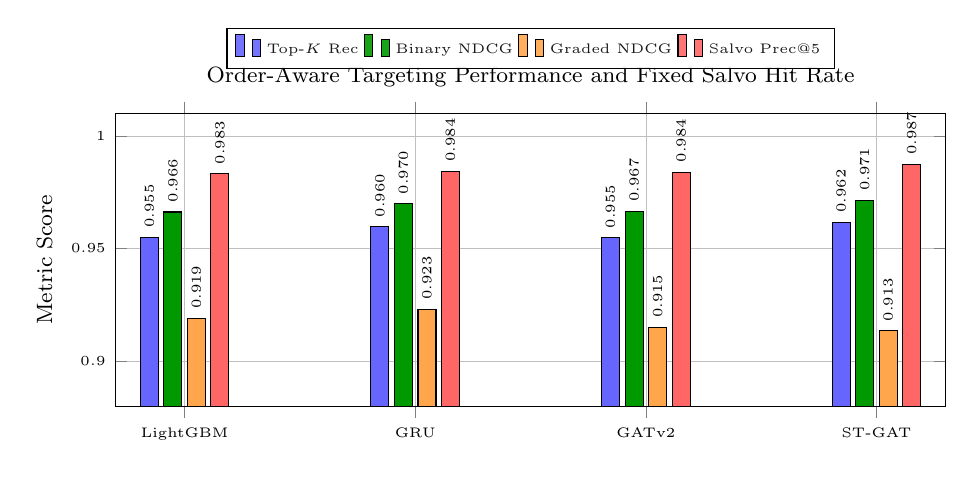
\begin{tikzpicture}
\begin{axis}[
    ybar,
    bar width=6.5pt,
    width=\columnwidth,
    height=5.3cm,
    ymin=0.88, ymax=1.01,
    ylabel={\footnotesize Metric Score},
    symbolic x coords={LightGBM, GRU, GATv2, ST-GAT},
    xtick=data,
    nodes near coords,
    nodes near coords style={font=\tiny, rotate=90, anchor=west},
    point meta=explicit symbolic,
    grid=both,
    grid style={line width=.1pt, draw=gray!20},
    major grid style={line width=.2pt,draw=gray!50},
    title={\footnotesize Order-Aware Targeting Performance and Fixed Salvo Hit Rate},
    label style={font=\tiny},
    tick label style={font=\tiny},
    legend style={at={(0.5,1.15)},anchor=south,legend columns=4,font=\tiny,fill=white,fill opacity=0.9}
]
\addplot[fill=blue!60] coordinates {(LightGBM,0.9550)[0.955] (GRU,0.9596)[0.960] (GATv2,0.9547)[0.955] (ST-GAT,0.9615)[0.962]};
\addplot[fill=green!60!black] coordinates {(LightGBM,0.9662)[0.966] (GRU,0.9698)[0.970] (GATv2,0.9665)[0.967] (ST-GAT,0.9712)[0.971]};
\addplot[fill=orange!70] coordinates {(LightGBM,0.9188)[0.919] (GRU,0.9230)[0.923] (GATv2,0.9148)[0.915] (ST-GAT,0.9134)[0.913]};
\addplot[fill=red!60] coordinates {(LightGBM,0.9831)[0.983] (GRU,0.9843)[0.984] (GATv2,0.9839)[0.984] (ST-GAT,0.9872)[0.987]};
\legend{Top-$K$ Rec, Binary NDCG, Graded NDCG, Salvo Prec@5}
\end{axis}
\end{tikzpicture}
\caption{Comparison of order-aware targeting metrics across all four architectures. Under a fixed 5-interceptor salvo ($K=5$), all models exceed $98.3\%$ precision, with ST-GAT leading at $98.72\%$.}
\label{fig:targeting_barchart}
\end{figure}

\subsubsection{Trajectory Invariance: The Flawless 1.0000 Agent-Level F1}
In operational deployment, a ground station tracks drones over continuous trajectories rather than isolated snapshots. When predicted probabilities are averaged across each drone's trajectory ($\bar{p}_i = \frac{1}{T_i} \sum_{t=1}^{T_i} p_i(t)$), both **GRU and ST-GAT achieve a flawless 1.0000 Agent-Level F1 score**. Across all 15 held-out scenarios containing hundreds of drone trajectories, zero whole-mission drone identity errors occurred.

\subsubsection{Mission Timeline Evolution and Field Promotions}
\cref{tab:timeline_and_promo} reports model behavior across mission phases and during in-flight dynamic role transitions.

\begin{table}[h]
\centering
\caption{Timeline Progression and Field Promotion Tracking}
\label{tab:timeline_and_promo}
\scriptsize
\resizebox{\columnwidth}{!}{%
\begin{tabular}{l c c c c}
\toprule
\textbf{Evaluation Dimension} & \textbf{LightGBM} & \textbf{GRU} & \textbf{GATv2} & \textbf{ST-GAT} \\
\midrule
$t=0$ Snapshot PR-AUC (Cold-Start) & $\mathbf{0.8966}$ & $0.5836$ & $0.6767$ & $0.7179$ \\
Early Mission PR-AUC ($0 - 33\%$) & $\mathbf{0.9850}$ & $0.9821$ & $0.9780$ & $0.9812$ \\
Mid Mission PR-AUC ($33 - 67\%$) & $0.9942$ & $\mathbf{0.9950}$ & $0.9915$ & $0.9938$ \\
Late Mission PR-AUC ($67 - 100\%$) & $\mathbf{0.9976}$ & $0.9964$ & $0.9949$ & $0.9960$ \\
\midrule
\textbf{Post-Promotion Recall ($0 \to 1$)} & $69.43\%$ & $\mathbf{82.06\%}$ & $62.38\%$ & $72.37\%$ \\
\bottomrule
\end{tabular}%
}
\end{table}

\begin{itemize}
    \item \textbf{The $t=0$ Cold-Start Dilemma:} At mission start ($t=0$), neural sequence models have empty history buffers (15 of GRU's 16 window slots are zero-padded), yielding $0.5836$ PR-AUC. In contrast, **LightGBM leads at $t=0$ ($0.8966$ PR-AUC)** because decision trees split directly on instantaneous spatial geometry (`dist_to_centroid`, `min_neighbor_dist`). However, within 8 timesteps ($0.8\text{ s}$), GRU and ST-GAT catch up completely ($>0.98$).
    \item \textbf{Dynamic In-Flight Promotions ($0 \to 1$):} When a critical commander is eliminated and an escort decoy is promoted to command, **GRU achieves the highest post-promotion recall ($82.06\%$)**. Its recurrent hidden state adapts quickly as the promoted drone moves toward the core, whereas purely spatial snapshot models (GATv2, $62.38\%$) struggle to reclassify newly promoted peripheral nodes.
\end{itemize}

\section{Operational Deployment Blueprint}
\label{sec:deployment}

Based on computational latency, memory footprint, and architectural characteristics, we outline an operational deployment blueprint mapping each model to its best defense tier (\cref{tab:deployment_matrix}).

\begin{table}[h]
\centering
\caption{Operational Counter-Swarm Deployment Matrix}
\label{tab:deployment_matrix}
\scriptsize
\begin{tabularx}{\columnwidth}{l l X}
\toprule
\textbf{Architecture} & \textbf{Profile \& Latency} & \textbf{Recommended Operational Role} \\
\midrule
\textbf{2-Layer GRU} 
& $0.06\text{ ms/agent}$ \newline $O(1)$ stream, low RAM 
& \textbf{Forward Interceptor UAVs:} Battery-powered edge platforms requiring minimum miss rate ($3.3\%$) and rapid adaptation to field promotions. \\
\midrule
\textbf{ST-GAT} 
& $18.5\text{ ms/step}$ \newline $T=8$ graph buffers 
& \textbf{Central Command Posts:} High-compute defense headquarters prioritizing maximum precision ($95.8\%$) and $98.7\%$ hit rate on fixed 5-shot salvos. \\
\midrule
\textbf{LightGBM} 
& $1.5\text{ ms/step}$ \newline 52D tabular vector 
& \textbf{Instant Cold-Start Defense:} Scenarios requiring immediate $t=0$ engagement upon launch, offline forensic analysis, or non-neural environments. \\
\midrule
\textbf{Spatial GATv2} 
& $3.8\text{ ms/step}$ \newline Single-frame graph 
& \textbf{Memoryless Interceptors:} Operational contexts where historical frame buffering is prohibited by policy or severe communication jitter. \\
\bottomrule
\end{tabularx}
\end{table}

\section{Conclusion and Future Work}
\label{sec:conclusion}

In this paper, we introduced an end-to-end, target-agnostic machine learning framework for critical agent identification in autonomous aerial swarms. By deriving 22 invariant kinematic, geometric, and dynamic graph features directly from downlinked position and velocity telemetry $(P, V)$, our approach operates with zero knowledge of enemy mission targets. Comprehensive benchmarking across 305,016 test observations demonstrated that both GRU and ST-GAT achieve a perfect $1.0000$ Agent-Level Trajectory F1, while directing fixed 5-missile salvos with a $98.72\%$ hit rate.

Future research will extend this framework to adversarial and contested environments, investigating robustness against radar line-of-sight occlusions, sensor noise, intermittent telemetry dropouts, and deliberate electronic warfare spoofing.

% -------------------------------------------------------------------------
% References
% -------------------------------------------------------------------------
\bibliographystyle{IEEEtran}
\bibliography{refs}

\end{document}
